\subsection{Prodotto matrice-matrice}
Il prodotto matrice-matrice è un algoritmo dell'algebra lineare che definisce la moltiplicazione tra due matrici. Esso produce una nuova matrice.
Formalmente, sia $A \in M_{m,n}, B \in M_{n,p}$, allora $A\cdot B = C$, dove $C \in M_{m,p}$.
La matrice risultante $C$ viene calcolato dal seguente algoritmo:
\begin{lstlisting}
for i from 0 to m do
    for j from 0 to n do
        C[i][j] = scalarProduct(A, B, i, j);
\end{lstlisting}
dove scalarProduct(A, B, i, j) é l'algoritmo per il prodotto scalare standard tra l'$i$-esima riga di A e la $j$-esima colonna di B.

\subsection{Approccio alla risoluzione}
La suddivisione del carico di lavoro sfrutterá la libreria openMPI, che implementa il message passing tra calcolatori di tipo MIMD a memoria distribuita.

Verrá supposto che le matrici A e B siano quadrate e di eguale dimensione. Inoltre, considereremo esclusivamente i casi in cui il numero di processi sia un divisore della dimensione delle matrici.

\subsection{Strategia di comunicazione}
Per l'algoritmo del prodotto matrice-matrice, sono possibili tre tipi di suddivisione del carico.
\begin{enumerate}
    \item Si suddivide la matrice A in blocchi di righe, B in blocchi di colonne.
    \item Si suddivide A in blocchi di colonne, B in blocchi di righe.
    \item Si suddividono A e B in blocchi di colonne.
    \item Si suddividono A e B in blocchi quadrati.
\end{enumerate}
Tra queste, é stata scelta la quarta, anche nota come algoritmo di Fox o BMR (Broadcast Multiply Roll).

In primis, disponiamo virtualmente i processi secondo una topologia a griglia. Adesso, un processo avrá un indice di riga e di colonna.

Dividiamo le matrici in blocchi quadrati: verranno create delle sottomatrici $A_{ij}$, $B_{ij}$, $C_{ij}$, che verranno assegnate ai processi in posizione $ij$ nella griglia.

Supponiamo di avere una griglia 3x3 di processi. Allora ciascuna matrice (A,B,C) verrá suddivisa in 9 sottomatrici.

Le sottomatrici di C potranno essere calcolate con le seguenti operazioni:
$C_{00} = A_{00}\cdot B_{00} + A_{01}\cdot B_{10} + A_{02}\cdot B_{20}$ \\
$C_{01} = A_{00}\cdot B_{01} + A_{01}\cdot B_{11} + A_{02}\cdot B_{21}$ \\
$C_{02} = A_{00}\cdot B_{02} + A_{01}\cdot B_{12} + A_{02}\cdot B_{22}$ \\
... \\
$C_{22} = A_{20}\cdot B_{02} + A_{21}\cdot B_{12} + A_{22}\cdot B_{22}$ \\


\begin{figure}[!htbp]
    \centering
    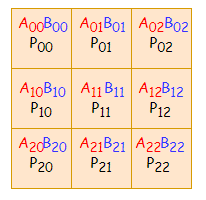
\includegraphics{distribuzioneIniziale.png}
    \caption{Distribuzione iniziale dei sottoblocchi di A e B}
    \label{fig:enter-label}
\end{figure}  
\begin{figure}[!htbp]
    \centering
    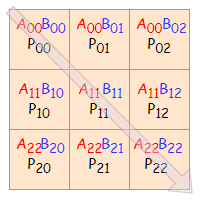
\includegraphics{primaDiagonale.png}
    \caption{Primo passo}
    \label{fig:enter-label}
\end{figure}  
\begin{figure}[!htbp]
    \centering
    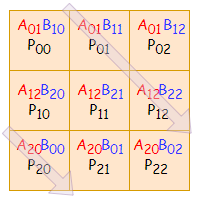
\includegraphics{secondaDiagonale.png}
    \caption{Secondo passo}
    \label{fig:enter-label}
\end{figure}  
\begin{figure}[!htbp]
    \centering
    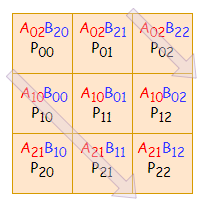
\includegraphics{terzaDiagonale.png}
    \caption{Terzo passo}
    \label{fig:enter-label}
\end{figure}  

Notiamo che, con questa disposizione delle sottomatrici, solo i processi sulla diagonale maggiore riusciranno a calcolare un contributo per la propria sottomatrice C di competenza. In particolare, notiamo che tutti i processi sulla stessa riga necessitano del sottoblocco B dell'elemento sulla diagonale. Quindi, condividiamo tale sottoblocco con tutti i processi sulla stessa riga, che adesso potranno calcolare un addendo della propria sottomatrice C.

Successivamente, notiamo che un processo in posizione i,j della griglia puó calcolare un altro addendo: 
\begin{itemize}
    \item richiedendo il sottoblocco B dal processo in posizione i-1,j, considerando peró la periodicitá delle dimensioni ($0 - 1 = 2$). Allora, effettuiamo una rotazione verticale verso l'alto dei sottoblocchi di B.
    \item richiedendo il sottoblocco A dal processo che si trova sulla diagonale che parte dalla posizione 01 (diagonale maggiore shiftata di 1 elemento verso destra). Quindi condividiamo tale sottoblocco con i processi della stessa riga.
\end{itemize}


Per calcolare l'ultimo addendo, dovremmo ripetere il passo precedente, ma shiftando un altra volta di una posizione verso destra la diagonale di riferimento.

A questo punto, avendo capito il pattern, generalizziamo l'algoritmo:
\begin{lstlisting}
    for k from 0 to p-1 do
        //controllo se sono un processo sulla diagonale attuale
        if coord_y = (coord_x+k)mod p then
            broadcast A_local to x-th row processes
        else
            receive into A_local_temp from process in position (coord_x, (coord_x+k)mod p)

        //effettuo il calcolo locale
        C_local = C_local + matrixProduct(A_local_temp, B_local)

        //ruoto verticalmente B
        send B_local to process in position ((coord_x-1)mod p, coord_y)
        receive into B_local from process in position ((coord_x+1)mod p, coord_y)
\end{lstlisting}